\documentclass[a4paper, 12pt,oneside]{article} 
%\documentclass[a4paper, 12pt,oneside,draft]{article} 

\usepackage{preamble}
\usepackage{bm}
%--------------------- ACTUAL FILE ---------------------- %
\begin{document} 
%%%
	%\thispagestyle{empty}
	%\vspace*{\fill}
	\begin{center}
	    \Large
	    \textbf{Orthogonalization Techniques for a Set of Vectors}
	        
	    \vspace{0.4cm}
	    \large
		HPC for numerical methods and data analysis \\
	    Student : Tara Fjellman \\
	    \small{Fall 2024}
	\end{center}
	\section{Introduction}
	QR factorization is a fundamental operation in numerical linear algebra. It is used in many applications, such least squares problems, computing the low rank approximation of a matrix, and computing an orthogonal basis of a set of vectors. It is defined as the factorization of a matrix $\mathbf{A}\in \mathbb{R}^{m \times n}$ into the product of an orthogonal matrix $\mathbf{Q}\in \mathbb{R}^{m \times n}$ and an upper triangular matrix $\mathbf{R}\in \mathbb{R}^{n \times n}$, such that $\mathbf{A} = \mathbf{Q} \mathbf{R}$. The QR factorization can be computed using different algorithms, such as Classical Gram-Schmidt (CGS), Cholesky-QR, and Tall-Skinny QR (TSQR). These algorithms have different numerical properties and computational costs, which makes them suitable for different applications. In this project, we study the numerical stability and computational performance of these algorithms for orthogonalizing a set of vectors. We will compare the algorithms using theoretical analysis and numerical experiments on different matrices. The goal is to identify an algorithm that is numerically stable and computationally efficient for orthogonalizing a set of vectors.

	In this project we make the assumption that $m \gg n$ and consider a couple of different forms for the $\mathbf{A}$ matrix. Typically we take $n$ between 50 and a few hundreds, while $m$ can be much larger.
	\section{Algorithms}
		\subsection{Classical Gram-Schmidt}
			Given a set of linearly independent vectors $\mathbf{a}_1, \ldots, \mathbf{a}_n \in \mathbb{R}^m$, the Gram-Schmidt algorithm computes an orthogonal basis $\mathbf{q}_1, \ldots, \mathbf{q}_n \in \mathbb{R}^m$ by orthogonalizing the vectors one by one. At the step $i$ of the algorithm, the $i$th vector $a_j$ is projected onto the orthogonal complement of the space spanned by the previous vectors $\mathbf{q}_1, \ldots, \mathbf{q}_{i-1}$, and the resulting vector is normalized to obtain $\mathbf{q}_i$.

			CGS is obtained by approximating the projector $I-Q(:,1:i)Q^\dagger(:,1:i)$ by $I-Q(:,1:i)Q^T(:,1:i)$. This corresponds to assuming $[Q(:,1:i)^TQ(:,1:i)]^{-1}=I$, i.e. that no numerical errors are committed during the orthogonalisation process. 
		\subsection{Cholesky-QR}
			The Cholesky-QR algorithm consists in computing $Q=AR^{-1}$ with $R$ found with help of the Cholesky decomposition of $A^TA$. The Cholesky decomposition of a matrix $\mathbf{G}$ is a factorization of the form $\mathbf{G} = \mathbf{L} \mathbf{L}^T$, where $\mathbf{L}$ is a lower triangular matrix. Indeed, the Cholesky decomposition $A^TA=LL^T$ gives $R=L^T$ since $(QR)^T(QR)=R^TR\iff Q^TQ=I$. 
			
			Notice that in practice, instead of inverting $R$ we can solve the system $R^TQ^T=A^T$ taking advantage of the triangular structure of $R$.
		\subsection{TSQR}
		% "explain why it minimizes communication,state the reduction tree used, state the algebra and the dimensions of intermediate Q factors."
		%Remember that communication refers to messages between processors. In the recent years we've seen trends causing floating point to become faster than communication. This is why it's important to minimize communication when dealing with parallelism.
		The TSQR, ``Tall Skinny QR'' algorithm is a communication avoiding algorithm for matrices with many more rows than columns. 
		To better understand how it works, we first explain it assuming we were using P = 4 processors, therefore scattering row wise our matrix $A$ along 4 processors $A_1, A_2, A_3, A_4 \in \mathbb{R}^{m / 4 \times n}$. We will then discuss how to go from this specific case to the more general one. 
		
		The computation can be expressed as a product of intermediate orthonormal factors in a binary tree like structure.

		At the leaves of the binary tree, we perform in parallel 4 local QR factorizations to get $A_1=\hat{Q}_1^{(2)} \hat{R}_1^{(2)}, A_2=\hat{Q}_2^{(2)} \hat{R}_2^{(2)}, A_3=\hat{Q}_3^{(2)} \hat{R}_3^{(2)}, A_4=\hat{Q}_4^{(2)} \hat{R}_4^{(2)}$. Here $\hat{Q}_l^{(2)} \in \mathbb{R}^{m / 4 \times m / 4}$ and $\hat{R}_l^{(2)} \in \mathbb{R}^{m / 4 \times n}$. In block structure we get
		$$
		\left[\begin{array}{l}
		A_1 \\
		A_2 \\
		A_3 \\
		A_4
		\end{array}\right]=\left[\begin{array}{llll}
		\hat{Q}_1^{(2)} & & & \\
		& \hat{Q}_2^{(2)} & & \\
		& & \hat{Q}_3^{(2)} & \\
		& & & \hat{Q}_4^{(2)}
		\end{array}\right]\left[\begin{array}{l}
		\hat{R}_1^{(2)} \\
		\hat{R}_2^{(2)} \\
		\hat{R}_3^{(2)} \\
		\hat{R}_4^{(2)}
		\end{array}\right]
		$$

		Recall that $\hat{R}_l^{(2)} \in \mathbb{R}^{m / 4 \times n}$ are tall and skinny upper triangular matrices, hence they can be written as
		$$
		\hat{R}_l^{(2)}=\left[\begin{array}{c}
		R_l^{(2)} \\
		0
		\end{array}\right]
		$$

		where $R_l^{(2)} \in \mathbb{R}^{n \times n}$. In the second level of the binary tree we combine the upper triangular matrices $R_1^{(2)}$ with $R_2^{(2)}$ and $R_3^{(2)}$ with $R_4^{(2)}$ to get block structured matrices. We perform the QR factorization in parallel to get the following structured matrices

		$$
		\left[\begin{array}{c}
		R_1^{(2)} \\
		R_{(2)}^{(2)}
		\end{array}\right]=\left[\begin{array}{cc}
		\hat{Q}_{11}^{(1)} & \hat{Q}_{12}^{(1)} \\
		\hat{Q}_{21}^{(1)} & \hat{Q}_{22}^{(2)}
		\end{array}\right]\left[\begin{array}{c}
		R_1^{(1)} \\
		0
		\end{array}\right] \quad\left[\begin{array}{l}
		R_3^{(2)} \\
		R_{(4)}^{(2)}
		\end{array}\right]=\left[\begin{array}{ll}
		\hat{Q}_{33}^{(1)} & \hat{Q}_{34}^{(1)} \\
		\hat{Q}_{43}^{(1)} & \hat{Q}_{44}^{(2)}
		\end{array}\right]\left[\begin{array}{c}
		R_3^{(1)} \\
		0
		\end{array}\right] .
		$$
		
		This can be written as
		$$
		\left[\begin{array}{c}
		\hat{R}_1^{(2)} \\
		\hat{R}_2^{(2)} \\
		\hat{R}_3^{(2)} \\
		\hat{R}_4^{(2)}
		\end{array}\right]=\left[\begin{array}{cccccccc}
		\hat{Q}_{11}^{(1)} & & \hat{Q}_{12}^{(1)} & & & & & \\
		& I & & & & & & \\
		\hat{Q}_{21}^{(1)} & & \hat{Q}_{22}^{(1)} & & & & & \\
		& & & I & & & & \\
		& & & & \hat{Q}_{33}^{(1)} & & \hat{Q}_{34}^{(1)} & \\
		& & & & & I & & \\
		& & & & \hat{Q}_{43}^{(1)} & & \hat{Q}_{44}^{(1)} & \\
		& & & & & & & I
		\end{array}\right]\left[\begin{array}{c}
		R_1^{(1)} \\
		0 \\
		R_3^{(1)} \\
		0
		\end{array}\right] .
		$$
		
		Finally at the root of the tree we compute the last QR factorization
		$$
		\left[\begin{array}{c}
		R_1^{(1)} \\
		R_3^{(1)}
		\end{array}\right]=\left[\begin{array}{ll}
		\hat{Q}_{11}^{(0)} & \hat{Q}_{13}^{(0)} \\
		\hat{Q}_{31}^{(0)} & \hat{Q}_{33}^{(0)}
		\end{array}\right]\left[\begin{array}{c}
		R_1^0 \\
		0
		\end{array}\right]
		$$


		Which can be written as

		$$
		\left[\begin{array}{c}
		R_1^{(1)} \\
		0 \\
		R_{(3)}^{(1)} \\
		0
		\end{array}\right]=\left[\begin{array}{llll}
		\hat{Q}_{11}^{(0)} & & \hat{Q}_{13}^{(0)} & \\
		& I & & \\
		\hat{Q}_{31}^{(0)} & & \hat{Q}_{33}^{(0)} & \\
		& & & I
		\end{array}\right]\left[\begin{array}{c}
		R_1^{(0)} \\
		0 \\
		0 \\
		0
		\end{array}\right] .
		$$

		$\hat{Q}$ is represented implicitly as the product of the intermediate orthogonal matrices as ${\hat Q}={\hat Q}^{(2)}{\hat Q}^{(1)}{\hat Q}^{(0)}$.

		In the more general case, where $A$ is distributed over $2^q$ processors, we would have $q+1$ levels in the binary tree. The matrix $Q^{(k)}$ associated to level $k$ would be composed of $2^{q-k}$ blocks of size $m/2^{q-k} \times m/2^{q-k}$, with structure 
		$$
		\left[\begin{array}{llll}
		\hat{Q}_{ij}^{(k)} & & \hat{Q}_{ij}^{(k)} & \\
		& I & & \\
		\hat{Q}_{ji}^{(k)} & & \hat{Q}_{jj}^{(k)} & \\
		& & & I
		\end{array}\right].
		$$
		Notice the communication is minimal as no data is duplicated and the reduction tree is used to combine the results of the local QR factorizations.
	\section{Parallelisation}
		For the parallelization, the matrix $\mathbf{A}$ is  row-distributed among processors. Each processor $i$ owns a block $\mathbf{A}_i$ with $i=1:n_{\text{procs}}$ (resp. $i=0:n_{\text{procs}}-1$ in \texttt{python}).

		%For each algorithm you should give their pseudo-code and explain it. You should also explain the communication routines used and why they are used. 
		\subsection{Classical Gram-Schmidt}
			In parallel CGS we split the projection of the $i$th vector across the processors. This however requires an allreduce operation as the projection involves the full columns of $Q$. The norm of the obtained projection is also all-reduced to compute the normalization factor, which is needed across processors. The pseudocode is given in \ref{fig:CGS-pseudocode}.   
			\begin{figure}[htb]       
				\centering             
					\vspace{0em}
					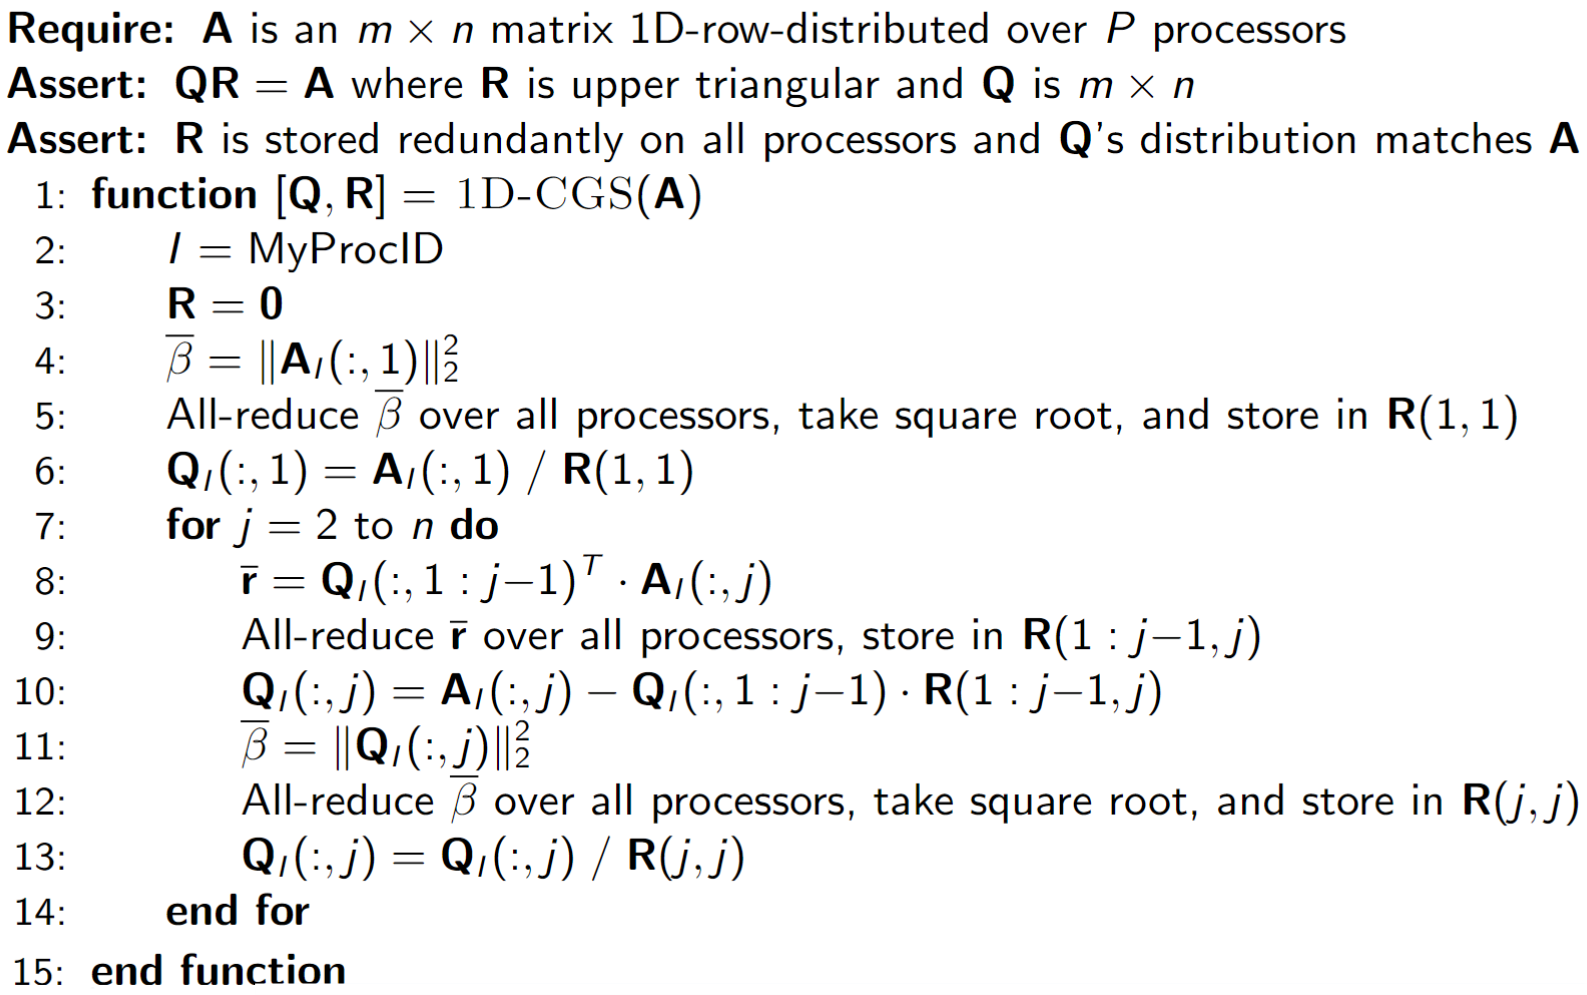
\includegraphics[width=.75\textwidth]{CGS_pseudocode}
					\caption{Pseudocode of parallelised CGS algorithm.}
					\label{fig:CGS-pseudocode}
			\end{figure}
		\subsection{Cholesky-QR}
			\begin{figure}
				\centering
				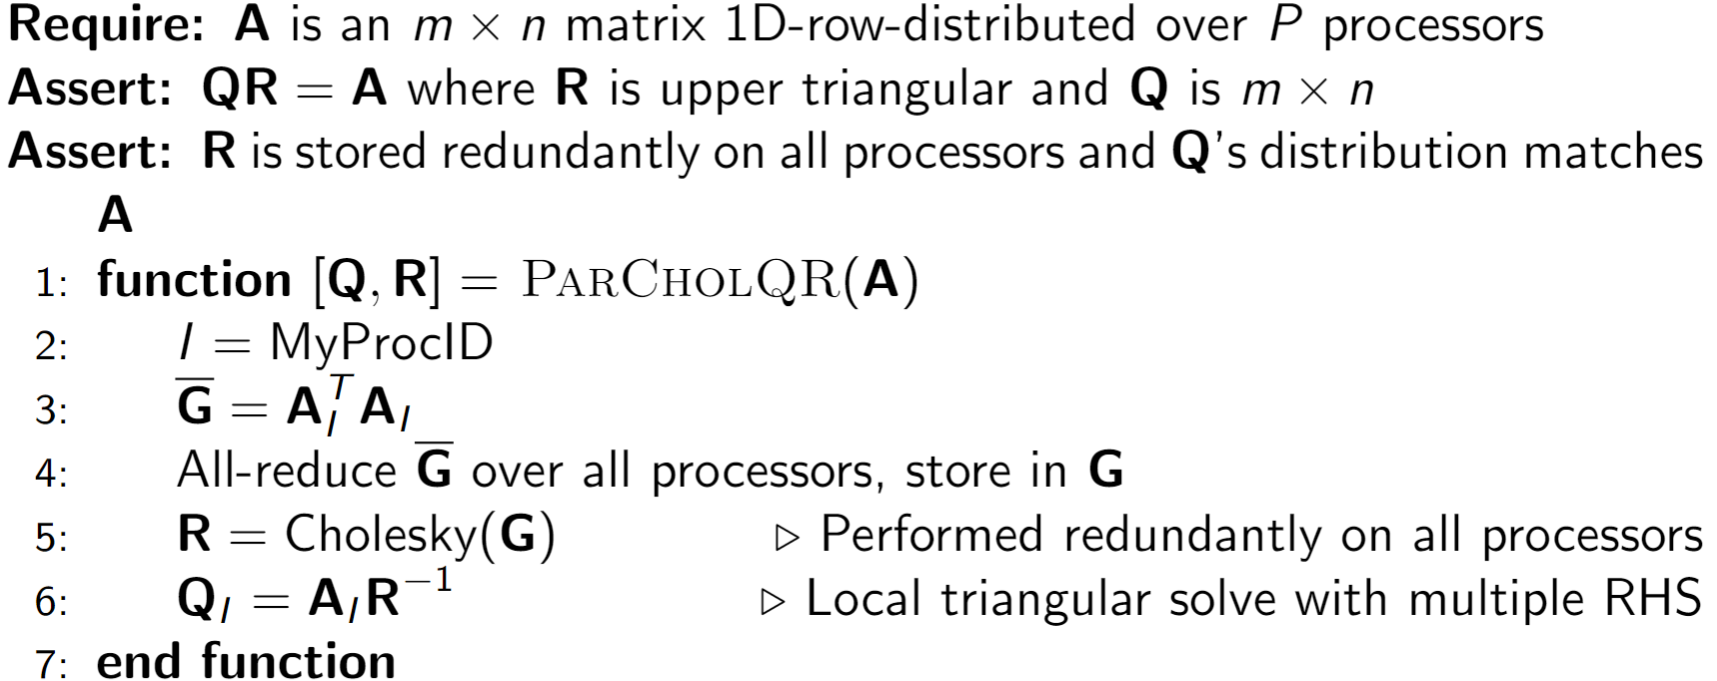
\includegraphics[width=.7\textwidth]{cholesky_QR_pseudocode}
				\caption{Pseudocode of parallelised Cholesky-QR algorithm.}
				\label{fig:Cholesky-QR-pseudocode}
			\end{figure}
		\subsection{TSQR}
			\begin{figure}
				\centering
				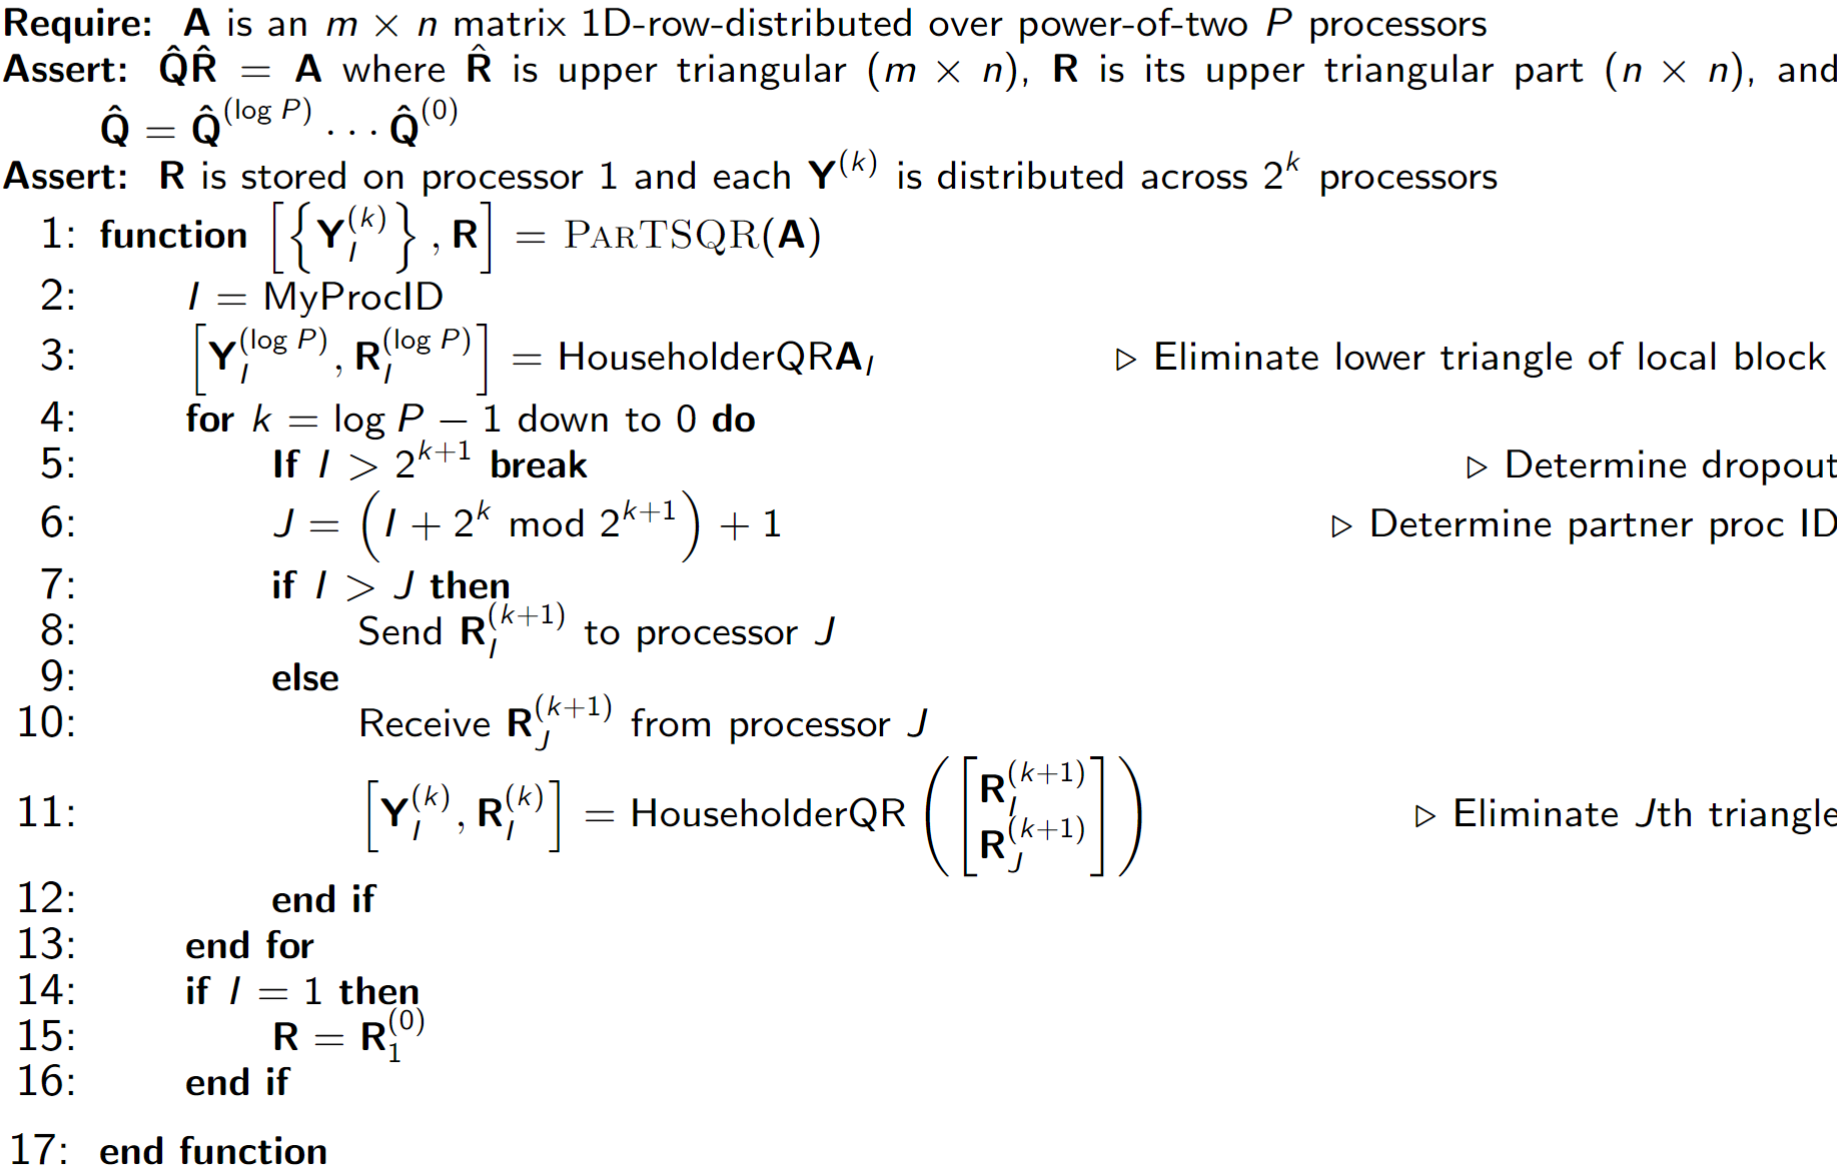
\includegraphics[width=.8\textwidth]{TSQR_pseudocode}
				\caption{Pseudocode of parallelised TSQR algorithm.}
				\label{fig:TSQR-pseudocode}
			\end{figure}
	
	\section{Experimental procedure}
		For a theoretical investigation, the bounds on the loss of orthogonality provided in the lectures should be used. For the numerical investigation, you should provide plots measuring the loss of orthogonality as $\left\|I-Q^T Q\right\|_2$ and the condition number of the basis $Q$. When it is possible, these quantities, along with the condition number of the input vectors, should be provided at each iteration of the algorithm when a new vector is orthogonalized. However this will not be possible for Cholesky-QR or TSQR for example. In this case you should present only the results obtained at the end of the algorithm.

		This investigation should be done on at least two different matrices. One of these matrices will be generated by uniformly discretizing a parametric function, also used in [1], that we denote $C \in \mathbb{R}^{m \times n}$. For all floating (and thus rational) numbers $0 \leq x, \mu \leq 1$, the function is defined as
		
		$$
		f(x, \mu)=\frac{\sin (10(\mu+x))}{\cos (100(\mu-x))+1.1}
		$$
		
		and the associated matrix is
		
		$$
		C \in \mathbb{R}^{m \times n}, \quad C(i, j)=f\left(\frac{i-1}{m-1}, \frac{j-1}{n-1}\right), i \in 1, \ldots, m, j \in 1, \ldots, n
		$$
		
		
		You could use for example $m=50000$ and $n=600$.
		Other matrices could be obtained for example from the SuiteSparse Matrix Collection, https: //sparse.tamu.edu/about. You can pick any square matrix, and then select only the first columns. The dimensions of the test matrices should be chosen such that you can compute the required quantities.
		
		Your report should state the theoretical bounds for the loss of orthogonality of the three algorithms. You should explain why these measures are important. For each matrix you should plot or put in a table the loss of orthogonality/condition number. You should explain these plots, reference them, and make connection with the theory.
	\section{Numerical Stability Investigation}
	\section{Runtime Investigation}
% Please add the following required packages to your document preamble:
% \usepackage{multirow}
\begin{table}[]
	\centering
	\begin{tabular}{|c|l|c|c|c|}
	\hline
	Metric                            & Matrix Type & Cholesky QR & Classical Gram-Schmidt & Tall-skinny     \\ \hline
	\multirow{2}{*}{$\|I-Q^TQ\|$}    & Non-singular A  & 100$\times 10^1$       & 100$\times 10^1$ & 100$\times 10^1$ \\ \cline{2-5} 
									  & Singular A      & 100$\times 10^1$       & 100$\times 10^1$ & 100$\times 10^1$ \\ \hline
	\multirow{2}{*}{$\kappa(Q)$} & Non-singular A  & 100$\times 10^1$       & 100$\times 10^1$ & 100$\times 10^1$ \\ \cline{2-5} 
									  & Singular A      & 100$\times 10^1$       & 100$\times 10^1$ & 100$\times 10^1$ \\ \hline
	\end{tabular}
	\caption{Metrics for numerical stability of the considered algorithms.}
	\label{tab:numberical-stability}
	\end{table}
	\section{Conclusion}
	\section*{Aknowledgements}
	%	\subsection{Time variation}
	%\section{Conclusion}
	%\section{Appendix}
	\appendix
		\section{Runtime Estimation}\label{appendix:runtime_estimation}
		%\input{elasticity_discussion.tex}	
	%\begin{figure}[htb]       % replace <line_nb> the with number of lines for the wrapping
	%	\centering                                          % and <side> by r or l for right or left (position on the page)
	%		\vspace{0em}
	%		\includegraphics[width=\textwidth]{yields_vs_T_for_diff_t}
	%		\caption{This is a caption}
	%		\label{fig:yield_vs_T_for_diff_t}
	%\end{figure}
	%\medskip
	%\titleformat*{\section}{\normalfont\large\bfseries}
	%\printbibliography[heading=bibintoc,title={Bibliography}] 
%	\vspace*{\fill}
%%%
\end{document} 